\documentclass[conference]{IEEEtran}
\usepackage{enumitem}
\usepackage{siunitx}
\usepackage{multicol}
\usepackage{array}
\usepackage{multirow}
\usepackage{adjustbox}
\usepackage[table]{xcolor}
\usepackage{colortbl}

\usepackage{caption}
\usepackage{amsfonts}
\usepackage{algorithm,algpseudocode}
\usepackage{lipsum}
\usepackage[flushleft]{threeparttable}

\usepackage{cite}
\usepackage{graphicx}
\graphicspath{{../../assets/}}
\usepackage{amsmath}
\usepackage{array}
\ifCLASSOPTIONcompsoc
 \usepackage[caption=false,font=normalsize,labelfont=sf,textfont=sf]{subfig}
\else
 \usepackage[caption=false,font=footnotesize]{subfig}
\fi
\usepackage{float}
\usepackage{url}

% \hyphenation{op-tical net-works semi-conduc-tor}

\usepackage{algorithm,algpseudocode}
\usepackage{lipsum}

\makeatletter
\newenvironment{breakablealgorithm}
  {% \begin{breakablealgorithm}
   \begin{center}
     \refstepcounter{algorithm}% New algorithm
     \hrule height.8pt depth0pt \kern2pt% \@fs@pre for \@fs@ruled
     \renewcommand{\caption}[2][\relax]{% Make a new \caption
       {\raggedright\textbf{\fname@algorithm~\thealgorithm} ##2\par}%
       \ifx\relax##1\relax % #1 is \relax
         \addcontentsline{loa}{algorithm}{\protect\numberline{\thealgorithm}##2}%
       \else % #1 is not \relax
         \addcontentsline{loa}{algorithm}{\protect\numberline{\thealgorithm}##1}%
       \fi
       \kern2pt\hrule\kern2pt
     }
  }{% \end{breakablealgorithm}
     \kern2pt\hrule\relax% \@fs@post for \@fs@ruled
   \end{center}
  }
\makeatother

\begin{document}
\title{Fast Parallel Image Rotation Algorithm}
\author {
    Dhrubajyoti Mandal \\
    \textit{School of Computer Engineering} \\
    \textit{Kalinga Institute of Industrial Technology} \\
    Bhubaneswar, India \\
    22053859@kiit.ac.in \\ \\ \\
    Sourav Kumar Parida \\
    \textit{School of Computer Engineering} \\
    \textit{Kalinga Institute of Industrial Technology} \\
    Bhubaneswar, India \\
    22051032@kiit.ac.in \\ \\
    Subhadeep Bhadra \\
    \textit{School of Computer Engineering} \\
    \textit{Kalinga Institute of Industrial Technology} \\
    Bhubaneswar, India \\
    2205336@kiit.ac.in
    \and
    Dr. Sujoy Dutta \\
    \textit{Asst. Prof. \& Asst. CoE} \\
    \textit{School of Computer Engineering} \\
    \textit{Kalinga Institute of Industrial Technology} \\
    Bhubaneswar, India \\
    sdattafcs@kiit.ac.in \\ \\
    Chiranjeev Bhaya \\
    \textit{Lead Engineer (Camera System)} \\
    \textit{Samsung R\&D Institute} \\
    Bangalore, India \\
    c.bhaya@samsung.com \\ \\
    Chandra Mohan V \\
    \textit{Architect (Camera System)} \\
    \textit{Samsung R\&D Institute} \\
    Bangalore, India \\
    chandra.mv@samsung.com
}
\maketitle
\begin{abstract}
    This paper presents a novel fast image rotation algorithm that leverages CPU parallelization while maintaining high image quality. The proposed method is a single-pass algorithm, derived from the existing Double-Line Rotation (DLR) method, which reduces computational complexity and generalizes the algorithm. Initially, a baseline for the given image is calculated to determine the starting line, which defines the initial point for each vertical or horizontal line in the image to be rotated. The corresponding pixels to be mapped are identified using floating point arithmetic, and trigonometric calculations are performed only once per line. This approach ensures precise image transformation with minimal computational overhead.
    \textit{Index terms:} Image rotation, line rotation image transform, double-line rotation (DLR), parallel image rotation.
\end{abstract}
\IEEEpeerreviewmaketitle
\section{Introduction}
2-D Image Rotation has a number of applications in digital photography and image processing like image matching, alignment, \cite{gaster2012heterogeneous} etc. Highly accurate image rotation is essential for certain image processing tasks such as feature extraction and matching. Whilst there are many state-of-the-art image rotation algorithms, they have limitations in terms of image quality and speed \cite{ashtari2015double} \cite{park2009accurate}.
Parallel algorithms for image processing aim to execute faster than sequential algorithms, however designing and scheduling a fast parallel image rotation is a challenge \cite{kwon2016study}.
The most straightforward, and perhaps the most well known approach to implement image rotation is by using the rotation matrix \cite{evans2001rotations}, as described here
$$\begin{bmatrix}
        x' \\
        y'
    \end{bmatrix} = \begin{bmatrix}
        x - cx \\
        y - cy
    \end{bmatrix} * \begin{bmatrix}
        cos(\theta) & -sin(\theta) \\
        sin(\theta) & cos(\theta)
    \end{bmatrix}$$\\
where, $\theta$ is the angle of rotation, $x'$ and $y'$ are the new coordinates of the rotated image, and $(cx, cy)$ is the center of the original image, which is treated as the axis of rotation.\\
Assuming the centre of rotation of the new image is $(cx', cy')$, the final new coordinates are:
$$\begin{bmatrix}
        x' \\
        y'
    \end{bmatrix} = \begin{bmatrix}
        x' + cx' \\
        y' + cy'
    \end{bmatrix}$$
\subsection{Subsection Heading Here}
Subsection text here.
\subsubsection{Subsubsection Heading Here}
Subsubsection text here.

% %%%%%%%%%%%%%%%%%%%%%%%%%%%%%%%%%%%%%%%%%%%%%%%%%%%%%%%%%%%%%%%%%%%%
\section{Literature Survey}
\subsection{Affine Transformation}
A basic idea in computer graphics and geometry, affine transformation is a linear mapping method that maintains straight lines, planes, and points. The capacity to carry out a variety of geometric operations, including translation, scaling, rotation, shearing, and reflection, is what defines an Affine transformation. These transformations are powerful and adaptable tools with a wide range of applications because they are defined mathematically by combining translations and linear transformations.

\subsubsection{Properties}

\begin{itemize}
  \item Linearity and Translation:  The transformation is composed of a linear transformation  Ax and a translation $\beta$.  This combination allows for a wide range of geometric transformations while preserving the structure of the space.

  \item Preservation of Collinearity and Ratios:  Affine transformations preserve the collinearity of points and the ratios of distances along parallel lines.

  \item Combining Transformations:  Multiple affine transformations can be combined into a single affine transformation by matrix multiplication and vector addition.
\end{itemize}

\section*{Mathematical Formulation}
Affine transformations can be described by a combination of linear transformations and translations. The general form of an affine transformation in two dimensions is:
$$ y=Ax+b $$

where
\begin{itemize}
  \item \(x = \begin{bmatrix} x \\ y \end{bmatrix}\) is the input coordinate vector.\\
  \item \(A\) is a \(2 \times 2\) matrix that represents the linear part of the transformation.\\
  \item \(b = \begin{bmatrix} t_x \\ t_y \end{bmatrix}\) is the translation vector.\\
\end{itemize}


For a rotation by an angle \(\theta\) around the origin, the matrix \(\mathbf{A}\) is:
$$
A = \begin{bmatrix} $$cos(\theta)$$ & - $$sin(\theta)$$ \\ $$sin(\theta)$$ & $$cos(\theta)$$ \end{bmatrix}
$$

To center the rotated image within its original dimensions, the translation values \(t_x\) and \(t_y\) are calculated as follows:

\section*{Calculations}

\subsection*{New Dimensions}
The new width and height of the rotated image are determined using trigonometric functions based on the rotation angle:
$$ newWidth = width \cdot |cos(\theta)| +height  \cdot |sin(\theta)| $$
$$ newHeight = width \cdot |sin(\theta)| + height \cdot |cos(\theta)| $$

\subsection*{Center Points}
$$
c_x = \frac{width}{2}, \quad c_y = \frac{height}{2}
$$
$$
newCx = \frac{newWidth}{2}, \quad newCy = \frac{newHeight}{2}
$$

\subsection*{Translation Values}
The translation values to center the rotated image within its new dimensions are:
$$
t_x = c_x - (newCx \cdot cos(\theta) - newCy \cdot sin(\theta))
$$
$$
t_y = c_y - (newCx \cdot sin(\theta) + newCy \cdot cos(\theta))
$$

Thus, the affine transformation matrix that includes rotation and translation is:

$$
T = \begin{bmatrix}
cos(\theta) & -sin(\theta) & t_x \\
sin(\theta) & cos(\theta) & t_y
\end{bmatrix}
$$

The new coordinates \((x', y')\) after applying the affine transformation are:

$$
\begin{bmatrix}
x' \\
y'
\end{bmatrix}
=
\begin{bmatrix}
cos(\theta) & -sin(\theta) & t_x \\
sin(\theta) & cos(\theta) & t_y
\end{bmatrix}
\begin{bmatrix}
x \\
y \\
1
\end{bmatrix}
$$
$$ x' = cos(\theta) \cdot x - sin(\theta) \cdot y + t_x $$
$$ y' = sin(\theta) \cdot x + cos(\theta) \cdot y + t_y $$

\subsection{Affine Transformation Algorithm}
The following algorithm demonstrates how to rotate an image by a specified angle using OpenCV:
\begin{itemize}
\item Get image dimensions (rows and cols)
\item Convert the angle from degrees to radians
\item Calculate new dimensions for the rotated image (new\_cols, new\_rows)
\item Create a new image (rotated) with the new dimensions, initialized to black
\end{itemize}

\begin{breakablealgorithm}
    \caption{Image Rotation using Affine Transformation}
    \begin{algorithmic}[1]
        \Procedure{rotate\_affine}{$...$}
        \State Compute $\alpha = \cos(\text{angle})$ and $\beta = \sin(\text{angle})$
        \State Compute the center coordinates of the original and new images:
        \State $c_x = \text{cols} / 2.0$
        \State $c_y = \text{rows} / 2.0$
        \State $new\_c\_x = \text{new\_cols} / 2.0$
        \State $new\_c\_y = \text{new\_rows} / 2.0$
        \State Define the rotation matrix elements:
        \State $m_{11} = \alpha$
        \State $m_{12} = \beta$
        \State $m_{13} = (1 - \alpha) \cdot \text{new\_c\_x} - \beta \cdot \text{new\_c\_x} + \text{c\_x} - \text{new\_c\_x}$
        \State $m_{21} = -\beta$
        \State $m_{22} = \alpha$
        \State $m_{23} = \beta \cdot \text{new\_c\_x} + (1 - \alpha) \cdot \text{new\_c\_y} + \text{c\_y} - \text{new\_c\_y}$

        \For{each pixel $y$ from 0 to $\text{new\_rows} - 1$}
            \For{each pixel $x$ from 0 to $\text{new\_cols} - 1$}
                \State Compute the corresponding coordinates $(x\_, y\_)$ in the original image:
                \State $x\_ = \text{round}(m_{11} \cdot x + m_{12} \cdot y + m_{13})$
                \State $y\_ = \text{round}(m_{21} \cdot x + m_{22} \cdot y + m_{23})$

                \If{$(x\_, y\_)$ is within the bounds of the original image}
                    \State Set the pixel value at $(x, y)$ in the new image to the value at $(x\_, y\_)$ in the original image
                \EndIf
            \EndFor
        \EndFor

        \State \Return{rotated}
        \EndProcedure
    \end{algorithmic}
\end{breakablealgorithm}


% %%%%%%%%%%%%%%%%%%%%%%%%%%%%%%%%%%%%%%%%%%%%%%%%%%%%%%%%%%%%%%%%%%%%
\section{Image Rotation using Hermite Expansion}

\subsection{Hermite Expansion Method}
The Hermite polynomial expansion is a technique used to approximate functions, including image rotation. By using Hermite polynomials, we can achieve smooth and accurate interpolation, which is especially useful for image processing tasks.

\subsubsection{Properties of Hermite Polynomials}
\begin{itemize}
    \item Orthogonal polynomials with respect to the weight function $e^{-x^2}$.
    \item Useful for approximating smooth functions due to their interpolation properties.
    \item Can handle both function values and derivatives, providing higher accuracy.
\end{itemize}

\subsection{Mathematical Formulation}
Hermite polynomials, denoted as $H_n(x)$, are a set of orthogonal polynomials that arise in probability, combinatorics, and numerical analysis. They are defined by the recurrence relation:

$$
H_{n+1}(x) = 2xH_n(x) - 2nH_{n-1}(x),
$$ with initial conditions $H_0(x) = 1$ and $H_1(x) = 2x$. 
These polynomials satisfy the orthogonality condition:
$$
\int_{-\infty}^{\infty} H_m(x)H_n(x)e^{-x^2}dx
$$

\subsection{Hermite Expansion}

A function $f(x)$ can be expanded in terms of Hermite polynomials as:
$$
f(x) = \sum_{n=0}^{\infty} c_n H_n(x) e^{-x^2/2},
$$

where $c_n$ are the expansion coefficients given by:
$$
c_n = \frac{1}{\sqrt{2^n n! \sqrt{\pi}}} \int_{-\infty}^{\infty} f(x) H_n(x) e^{-x^2/2} dx.
$$


\subsection{Application of Hermite Expansion in Image Rotation}

The use of Hermite expansion in image rotation leverages the orthogonality of Hermite polynomials to approximate the image function. Given an image $I(x,y)$, it can be expanded using two-dimensional Hermite polynomials $H_{m,n}(x,y)$ as:
$$
I(x,y) = \sum_{m=0}^{\infty} \sum_{n=0}^{\infty} c_{m,n} H_m(x) H_n(y) e^{-(x^2 + y^2)/2},
$$
where $c_{m,n}$ are the expansion coefficients. These coefficients are computed as:
$$
c_{m,n} = \frac{1}{\sqrt{2^{m+n} m! n! \pi}} \int_{-\infty}^{\infty} \int_{-\infty}^{\infty} I(x,y) H_m(x) H_n(y) e^{-(x^2 + y^2)/2} dx dy.
$$

To rotate the image, the coordinates $(x,y)$ are transformed to $(x', y')$ as previously defined:
$$
\begin{bmatrix}
x' \\
y'
\end{bmatrix}
=
\begin{bmatrix}
cos \theta & -sin \theta \\
sin \theta & cos \theta
\end{bmatrix}
\begin{bmatrix}
x \\
y
\end{bmatrix}.
$$

\subsubsection{Finding Transformed Coordinates Using Hermite Expansion}

To find the transformed coordinates $(x', y')$ using Hermite expansion, we perform the following steps:

Expand the Image Function Using Hermite Polynomials:
    Given an image $I(x,y)$, we first expand it using the two-dimensional Hermite polynomials $H_{m,n}(x,y)$:
    $$
    I(x,y) = \sum_{m=0}^{\infty} \sum_{n=0}^{\infty} c_{m,n} H_m(x) H_n(y) e^{-(x^2 + y^2)/2}
    $$
    where the coefficients $c_{m,n}$ are determined using:
    $$
    c_{m,n} = \frac{1}{\sqrt{2^{m+n} m! n! \pi}} \int_{-\infty}^{\infty} \int_{-\infty}^{\infty} I(x,y) H_m(x) H_n(y) e^{-(x^2 + y^2)/2} dx dy.
    $$

Compute the Rotated Coordinates:
   Using the rotation matrix, we transform the coordinates $(x,y)$ to $(x',y')$:
   $$
   \begin{bmatrix}
   x' \\
   y'
   \end{bmatrix}
   =
   \begin{bmatrix}
   cos \theta & -sin \theta \\
   sin \theta & cos \theta
   \end{bmatrix}
   \begin{bmatrix}
   x \\
   y
   \end{bmatrix}.
   $$

Reconstruct the Rotated Image:
   The rotated image $I'(x',y')$ is reconstructed using the inverse Hermite expansion:
   $$
   I'(x',y') = \sum_{m=0}^{\infty} \sum_{n=0}^{\infty} c_{m,n} H_m(x') H_n(y') e^{-(x'^2 + y'^2)/2},
   $$
   where $H_m(x')$ and $H_n(y')$ are the Hermite polynomials evaluated at the transformed coordinates $(x', y')$.

By following these steps, the image can be rotated accurately using the Hermite expansion. This method ensures that the transformation leverages the orthogonality and interpolation properties of Hermite polynomials, resulting in a smooth and precise image rotation.


%%%%%%%%%%%%%%%%%%%%%%%%%%%%%%%%%%%%%%%%%%%%%%%%%%%%%%%%%%%%%%%%%%%%%%%%%%%%%%%%%%%%%%%%%%%%%%%%%%%%%%%%%%%%%%%

\section{Image Rotation using Double Line Rotation}

The Double Line Rotation (DLR) method is an innovative algorithm for fast image rotation, 
introduced to address the inefficiencies in traditional rotation techniques. 
The DLR method is based on the concept of dividing the image into multiple zones, 
each processed differently to achieve an efficient and accurate rotation.

\subsection{Methodology}

The DLR method divides the image into eight distinct zones, each characterized by 
specific rotation equations and transformations. The main idea is to map each pixel 
from the original image to two corresponding pixels in the target image, ensuring that 
the distance ratio between points remains constant throughout the rotation process. 
This is particularly useful in preserving the intensity and shape of the pixels, 
making the DLR method suitable for applications requiring invariant feature extraction.

\subsection{Zone Concepts}

The image is divided into the following zones:

\subsubsection{Zone 1}
In Zone 1, horizontal lines are used for rotation, and the slope of \( f_s(x) \) is positive. Each horizontal line in the original image \( T \) lies in a line with slope \( \tan(\alpha) \) and shears using the line \( f_s(x) = \left(\tan \alpha + \frac{\pi}{2}\right)x \). The size of the rotated image is calculated using:
\[
m_{rt} = \gamma_m + m, \quad n_{rt} = \gamma_n + n
\]
where \( \gamma_n = f_s(m) \rightarrow \left\| \frac{m}{\tan(\alpha + \frac{\pi}{2})} \right\| \) and \( \gamma_m = f(n) \rightarrow \| n \tan \alpha \| \).

\subsubsection{Zone 2}
In Zone 2, vertical lines are used for rotation, and the slope of \( f(y) \) is positive. The size of the rotated image is calculated similarly to Zone 1, but the vertical and horizontal lines are interchanged.

\subsubsection{Zone 3}
In Zone 3, the slope is negative, but the equations are the same as for Zone 2. Vertical lines are used, and the size of the rotated image \( R (m_{rt} \times n_{rt}) \) is calculated as follows:
\[
m_{rt} = \gamma_m + n, \quad n_{rt} = \gamma_n + m
\]
where \( \gamma_n = |f_s(n)| \rightarrow f_s(y) = \frac{y}{-\tan \alpha} \) and \( \gamma_m = \sqrt{m^2 - AC^2} \) in \( \triangle ABC \).

\subsubsection{Zone 4}
In Zone 4, horizontal lines are used, and the slope of \( f_s(x) \) is positive, but \( f(x) \) has a negative gradient. This means that lines are moving upwards, the original image's lines are sloping downwards. Each horizontal line in image \( T \) is mapped and similarly to Zone 1. The involves altering the position of each pixel along the horizontal lines according to the function 
\[
f_s(x) = \left(\tan \alpha + \frac{\pi}{2}\right)x.
\]

\subsubsection{Zone 5}
Zone 5 employs logical transformations on indices to generate the rotated image. These transformations involve manipulation of pixel positions such as swaps, inversionsof indices. The goal is to create a rotated image that retains the original dimensions while applying a different logical structure to the pixel arrangement. All zones are transformed, depending on whether vertical or horizontal lines are used. The size of the rotated image in Zone 1 and Zone 5 are the same, ensuring consistency in image dimensions.

\subsubsection{Zone 6}
Zone 6 is generated by transforming either Zone 2 or Zone 3. 
The transformation maintains the size of the rotated image and applies internal line transformations. These internal line transformations may include skewing, scaling, or shifting along specific axes to emphasize certain internal features. 

\subsubsection{Zone 7}
Zone 7, similar to Zone 6, is a transformation of other zones but uses vertical lines. The vertical line transformations involve modifying the image along the vertical axis, affecting the height of the image without altering its width. This vertical stretching or compressing highlights vertical patterns and structures within the image.
\subsubsection{Zone 8}
Zone 8 utilizes transformations from horizontal lines, similar to Zones 1 and 4. These horizontal transformations involve scaling operations that modify the image along the horizontal axis. The transformations in Zone 8 ensure that the overall balance of the image is maintained while providing a comprehensive view of horizontally oriented features.

\subsection{Calculation of the Base-Line, Start-Line, and Target Image Size}

The first step in the DLR method is calculating the target image size. Each zone uses specific equations to determine the size of the target image, ensuring accurate and efficient rotation. For example, in Zone 3:
\[
\gamma_n = \left| f_s(n) \right| \rightarrow f_s(y) = \frac{y}{-\tan \alpha}, \quad \gamma_m = \sqrt{m^2 - AC^2}
\]
where \( AC = (\cos \phi)m \) and \( \phi = (\pi - \alpha) - \frac{\pi}{2} \).

By dividing the image into zones and applying the DLR method, 
the rotation process becomes more efficient and accurate, 
preserving the original image's intensity and shape.




%%%%%%%%%%%%%%%%%%%%%%%%%%%%%%%%%%%%%%%%%%%%%%%%%%%%%%%%%%%%%%%%%%%%%%%%%%%%%%%%%%%%%%%%%%%%%%%%%%%%%%%%%%%5





\section{Proposed Method}
The proposed method is a single pass algorithm, which means that it performs the entire image rotation operation at once. The proposed algorithm predominantly affects pixels in the row major (width), or ones in the column major (height), depending on the angle of rotation, $\alpha$.
If $\alpha \in \left ( \frac{\pi}{4}, \frac{3 \pi}{4} \right ] \bigcup \left ( \frac{5 \pi}{4}, \frac{7 \pi}{4} \right ]$, rotation is performed in the \textit{\textbf{column major}}, and it is performed in the \textit{\textbf{row major}} for the rest of the angles. Accordingly, for rotating the source image, entire row or column vectors of pixels are rotated as a single unit, instead of the more common approach, where each individual pixel is separately mapped. Due to this reason, it is necessary to accurately determine the initial coordinates from which the new row or column vector will begin. The coordinates of the rest of the pixels in the vector can then be determined by simple floating point addition or subtraction, depending on the extent to which each of the said vectors are spread across the coordinate axes.

Apart from this, depending on $\alpha$, the pixel processing order changes - i.e., whether the last row or column vector of pixels get processed first, or last. Since it has been found out that these values are very sensitive to $\alpha$, the specific details of which are discussed in the later parts of this paper.
\subsection{Rotation Of An Image In The Column Major} \label{col_major_rotation}
\begin{figure}[H]
    \centering
    \captionsetup{justification=centering,margin=0.7cm}
    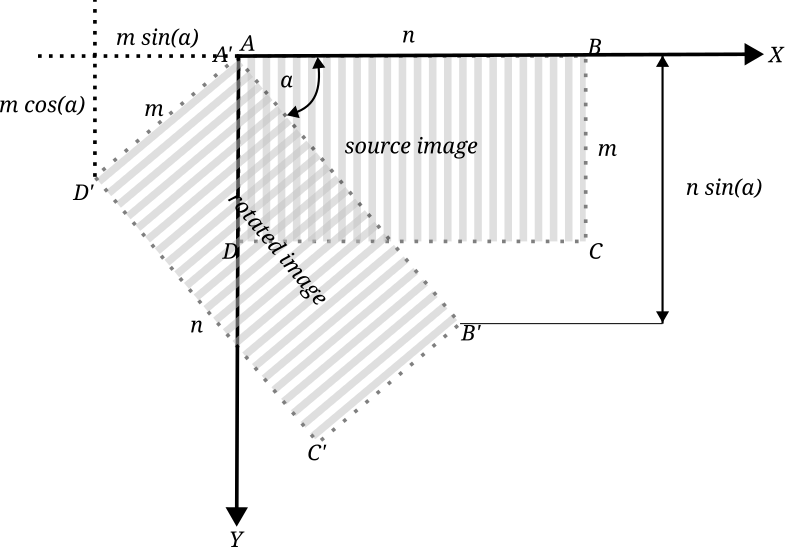
\includegraphics[width=0.5\textwidth]{rotation_example_1.png}
    \caption{Example demonstrating rotation of an image in the column major. Every column vector of pixels are rotated at once (Represented by the stripes in the image).}
    \label{fig:rotation_example_1}
\end{figure}
As seen in the example image in figure \ref{fig:rotation_example_1}, for the given angle of rotation, column vectors were rotated (represented by the stripes). Each such vector to be rotated begins from the line $\overrightarrow{A'B'}$. As such, the initial coordinates of each of these vectors can be determined by the equation of the same line, which is given by:
\begin{equation}
    \label{start_line_eq}
    f(i) = \left\lfloor \frac{i}{tan(\alpha)} \right\rfloor \forall \{i \in \mathbb{Z},\> i \in \left[ 0, n \cdot sin(\alpha) \right)\}
\end{equation}
Thus, the initial coordinates of the column vectors would be of the type $(f(i), i)$. Next, to determine the coordinates of the rest of the pixels in the column vector, as mentioned previously, we perform floating point addition or subtraction, depending on the extent to which each of the said vectors are spread across the coordinate axes.\\
In the example in figure \ref{fig:rotation_example_1}, we can see that each column vector is spread through a length of $m \cdot \sin(\alpha)$ in the $x$-axis and through a length of $m \cdot \cos(\alpha)$ in the $y$-axis. It may also be observed that these values are the projections of any line perpendicular to line defined by the function in equation \ref{start_line_eq} on the coordinate axes.\\
We now define:
$$\delta x = \left\lvert sin(\alpha)\right\rvert$$
$$\delta y = \left\lvert cos(\alpha)\right\rvert$$
The coordinates of the next pixel in the column vector is then given by:
$$(f(i) + \delta x, i + \delta y)$$
The coordinates of the pixel following that is determined by adding $\delta x$ and $\delta y$ to the previous coordinates accordingly, and so on, for each of the $m$ pixels in the given column vector. The end-result is that this operation covers all the $m \cdot \sin(\alpha)$ pixels in the $x$-axis and all the $m \cdot \cos(\alpha)$ pixels in the $y$-axis, therefore mapping all of the $m$ pixels in the specific column vector.\\
This process continues for all of the $n$ column vectors in the image, until the entire image is rotated. In practice, each column vector is actually mapped \textbf{twice}. The first mapping happens from the $i\>th$ column vector in $I$ to the $i\>th$ column vector in $R$. The second mapping happens from the $i\>th$ column vector in $I$ to the $(i+1)\>th$ column vector in $R$. Each of these $(i+1)\>th$ column vectors get overwitten in each iteration with a new column vector in $I$; however, this gives a sufficiently accurate issusion of anti-aliasing without losing much quality.

The signs for $\delta x$ and $\delta y$ depend on whether, while mapping the column vectors in the rotated image, the values of the $x$-coordinate $y$-coordinate are decreasing or increasing. In the given example in figure \ref{fig:rotation_example_1}, $\delta x$ is negative, but $\delta y$ is positive.\\
There is a third parameter, defined as:
$$\delta i = \frac{1}{\delta x}$$
$\delta i$ determines the rate at which the column vector is processed from one to the next, and its sign depends on the angle of rotation, $\alpha$.
The calculations for $\delta x$, $\delta y$, and $\delta i$ only happen once per column vector in the image, so the entire image transformation is quite fast, overall.
\subsection{Rotation Of An Image In The Row Major} \label{row_major_rotation}
\begin{figure}[H]
    \centering
    \captionsetup{justification=centering,margin=0.7cm}
    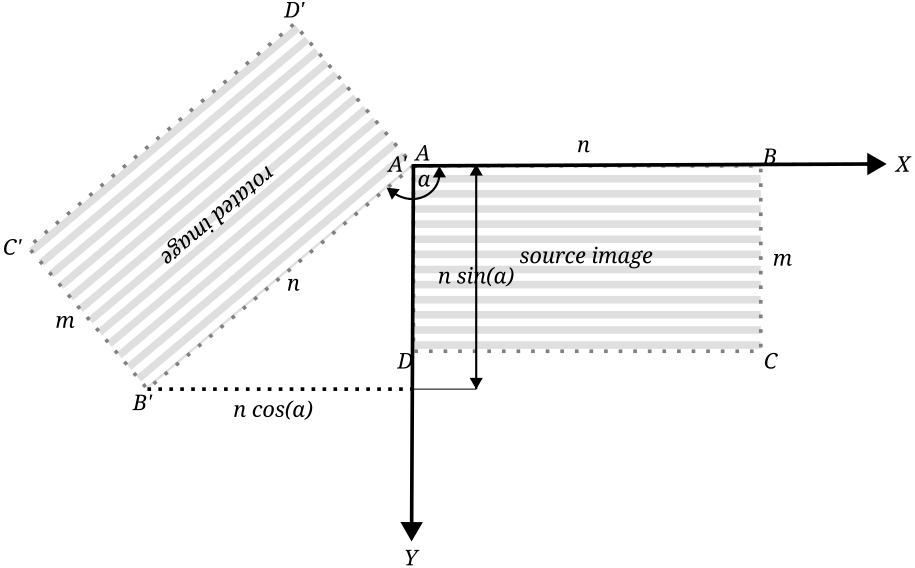
\includegraphics[width=0.5\textwidth]{rotation_example_2.png}
    \caption{Example demonstrating rotation of an image in the row major. Every row vector of pixels are rotated at once (Represented by the stripes in the image).}
    \label{fig:rotation_example_2}
\end{figure}
In the example image in figure \ref{fig:rotation_example_2}, for the given angle of rotation, row vectors were rotated (represented by the stripes). All the calculations and logic is very similar to the one described for rotation in the column major [\ref{col_major_rotation}]. Here, each vector to be rotated begins from the line $\overrightarrow{A'D'}$, whose equation is given by:
\begin{equation}
    \label{start_line_eq_2}
    f(i) = \left\lfloor \frac{i}{tan(\alpha + \frac{\pi}{2})} \right\rfloor \forall \{i \in \mathbb{Z},\> i \in \left[ 0, m \cdot cos(\alpha) \right)\}
\end{equation}
Everything else stays the same, except the fact that now, each row vector is spread through a length of $n \cdot \cos(\alpha)$ in the $x$-axis and through a length of $n \cdot \sin(\alpha)$ in the $y$-axis, and accordingly, we have:
$$\delta x = \left\lvert cos(\alpha)\right\rvert$$
$$\delta y = \left\lvert sin(\alpha)\right\rvert$$


\begin{table}[t]
    \begin{threeparttable}
        \caption{Notation}
        \label{table:notations}
        \centering
        \begin{tabular}{|m{1.5cm}|m{6cm}|}
            \hline
            \textbf{Symbol}  & \textbf{Description}                                                                                                                        \\
            \hline
            $I$              & Original image                                                                                                                              \\ \hline
            $m, n$           & Height, width of $I$                                                                                                                        \\ \hline
            $R$              & Rotated image                                                                                                                               \\ \hline
            $m', n'$         & Height, width of $R$                                                                                                                        \\ \hline
            $\alpha$         & Angle of rotation in radians                                                                                                                \\ \hline
            $x'$             & Offset by which the $x$-coordinates of $R$ need to be shifted                                                                               \\ \hline
            $y'$             & Offset by which the $y$-coordinates of $R$ need to be shifted                                                                               \\ \hline
            $f(...)$         & Function defining the equation of the line from where the row or column vector starts [eq. \ref{start_line_eq}] [eq. \ref{start_line_eq_2}] \\ \hline
            $r_o$            & Upper limit of the function $f$                                                                                                             \\ \hline
            $N$              & Number of elements (pixels) in the row or column vector $f$                                                                                 \\ \hline
            \verb|flip|      & Boolean value that changes pixel processing order based on $\alpha$                                                                         \\ \hline
            \verb|row_major| & Boolean value that determines whether processing is to be done in the row or column major                                                   \\ \hline
            \verb|negate|    & Boolean value, that if true, negates the indices used for indexing the pixels of the image                                                  \\ \hline
        \end{tabular}
        \begin{tablenotes}
            \small
            \item \textbf{Note:} The algorithm described in [Algorithm \ref{rotation_alorithm}] follows \textbf{\textit{Python}} style indexing. For example, if \verb|a = [[1, 2, 3], [5, 6]]|, then \verb|a[0][-1]| represents the element \verb|3|.
        \end{tablenotes}
    \end{threeparttable}
\end{table}


\subsection{Implementation}

\begin{breakablealgorithm} \label{rotation_alorithm}
    \caption{Image Rotation Algorithm}
    \begin{algorithmic}[1]
        \Procedure{rotate}{$...$}\Comment{Performs image rotation on $R$}
        \State \texttt{src\_i} $ = 0$ \Comment{Initialize internal control variables}
        \State \texttt{S} $ = 1$
        \State $M = [\>]$
        \If{\texttt{negate}}
        \State \texttt{S = -1}
        \EndIf

        \If{\texttt{flip}}
        \State $M = [m_i]\> for\> i=0,1,…,N-1,\>|\> m_i=N-i$
        \Else
        \State $M = [m_i]\> for\> i=0,1,…,N-1,\>|\> m_i=N$
        \EndIf

        \For{$i=0$ to $r_o$}
        \State \texttt{temp\_x = } $f(i)$
        \State \texttt{temp\_y = } $i$

        \For{$px$ in $M$}
        \State $x = \lfloor$ \texttt{temp\_x} $\rfloor$
        \State $y = \lfloor$ \texttt{temp\_y} $\rfloor$
        \State \texttt{temp\_i} $= \lfloor$ \texttt{src\_i} $\rfloor$

        \If{\texttt{row\_major}}
        \State $a = $ \texttt{temp\_i}
        \State $b = px$
        \Else
        \State $a = px$
        \State $b = $ \texttt{temp\_i}
        \EndIf

        \Comment{Map rotated pixels to $R$}
        \State $R[$ \texttt{S} $*\> (y + y'),\> $\texttt{ S }$ *\> (x + x')] = I[a, b]$
        \State $R[$ \texttt{S} $*\> (y + y') + 1,\> $\texttt{ S }$ *\> (x + x')] = I[a, b]$

        \State \texttt{temp\_x += } $\delta x$
        \State \texttt{temp\_y += } $\delta y$

        \EndFor

        \State \texttt{src\_i += } $\delta i$
        \EndFor

        \EndProcedure
    \end{algorithmic}
\end{breakablealgorithm}


The algorithm described above [Algorithm \ref{rotation_alorithm}] rotates image $I$ to $R$.\\
$R$ is Initialized as a blank image of width $n'$ and height $m'$ to fit $R$ in the canvas, where:
$$m' = \left\lceil \left\lvert m \cdot cos(\alpha) + n \cdot sin(\alpha) \right\rvert \right\rceil $$
$$n' = \left\lceil \left\lvert m \cdot sin(\alpha) + n \cdot cos(\alpha) \right\rvert \right\rceil $$
The rotation function is then invoked, with each of the parameters updating depending on the value of $\alpha$, as discussed above. The detailed values of each of the parameters are mentioned in [Table \ref{table:rotation_params}].\\ \\
\textbf{Note:} It has been observed, that for ranges of $\alpha$ which are vertically opposite each other (For example, angles in the range $\left ( \frac{\pi}{4}, \frac{\pi}{2} \right ]$ are vertically opposite angles in the range $\left ( \frac{5 \pi}{4}, \frac{ 3 \pi}{2} \right ]$, and so on), the only parameters of rotation that change are $\delta i$, \texttt{negate}, and \texttt{flip}. As such, the calculations have been generalized for such angles and they have been represented in [Table \ref{table:rotation_params}], with a $(')$ at the end of their names (shaded cells).\\


\begin{breakablealgorithm} \label{driver_function}
    \caption{Driver Function}
    \begin{algorithmic}[1]
        \Procedure{main}{$...$}\Comment{Invokes [Algorithm \ref{rotation_alorithm}]}

        \State Determine the boolean value of \texttt{row\_major}
        \State Determine \textit{\textbf{f}}, based on the value of \texttt{row\_major}
        \State Initialize a blank image $R$ with dimensions $(m', n')$

        \State Determine the parameters of rotation from [Table \ref{table:rotation_params}]

        \State Generate $R$ using [Algorithm \ref{rotation_alorithm}]
        \EndProcedure
    \end{algorithmic}
\end{breakablealgorithm}

\renewcommand{\arraystretch}{3}  % This sets the row height to 3 cm
\definecolor{lightgray}{gray}{0.91}
\begin{table*}[h]
    \caption{Rotation Parameters, based on $\alpha$}
    \label{table:rotation_params}
    \centering
    \begin{tabular}{ |p{0.8cm}|p{1.53cm}|p{1.53cm}|p{1.1cm}|p{1.1cm}|p{0.67cm}|p{1.53cm}|p{0.1cm}|p{0.87cm}|p{0.87cm}|>{\columncolor{lightgray}}p{0.67cm}|>{\columncolor{lightgray}}p{0.95cm}|>{\columncolor{lightgray}}p{0.8cm}| }
        \hline
        \raisebox{0ex}{\multirow{2}{*}{\adjustbox{angle=90}{\textbf{Range of $\alpha$}}}} & \multicolumn{12}{c|}{\textbf{Rotation parameters}}                                                                                                                                                                                                                                                                                                                                                                                                    \\
        \cline{2-13}
                                                                                          & \textbf{$x'$}                                                            & \textbf{$y'$}                                                            & \textbf{$\delta x$}                      & \textbf{$\delta y$}                      & \textbf{$\delta i$} & \textbf{$r_o$}                                                           & \textbf{N} & \texttt{negate} & \texttt{flip}  & \textbf{$\delta i'$} & \texttt{negate'} & \texttt{flip'} \\
        \hline
        $\left [ 0, \frac{\pi}{4} \right ]$                                               & $\left\lceil \left\lvert m \cdot \sin(\alpha) \right\rvert \right\rceil$ & 0                                                                        & $\left\lvert \cos(\alpha) \right\rvert$  & $\left\lvert \sin(\alpha) \right\rvert$  & $1 / \delta x$      & $\left\lceil \left\lvert m \cdot \cos(\alpha) \right\rvert \right\rceil$ & n          & \texttt{false}  & \texttt{false} & $1 / \delta x$       & \texttt{true}    & \texttt{false} \\
        \hline
        $\left ( \frac{\pi}{4}, \frac{\pi}{2} \right ]$                                   & $\left\lceil \left\lvert m \cdot \sin(\alpha) \right\rvert \right\rceil$ & 0                                                                        & $-\left\lvert \sin(\alpha) \right\rvert$ & $\left\lvert \cos(\alpha) \right\rvert$  & $-1 / \delta x$     & $\left\lceil \left\lvert n \cdot \sin(\alpha) \right\rvert \right\rceil$ & m          & \texttt{false}  & \texttt{false} & $1 / \delta x$       & \texttt{false}   & \texttt{true}  \\
        \hline
        $\left ( \frac{\pi}{2}, \frac{3 \pi}{4} \right ]$                                 & $m'$                                                                     & $\left\lceil \left\lvert m \cdot \cos(\alpha) \right\rvert \right\rceil$ & $-\left\lvert \sin(\alpha) \right\rvert$ & $-\left\lvert \cos(\alpha) \right\rvert$ & $-1 / \delta x$     & $\left\lceil \left\lvert n \cdot \sin(\alpha) \right\rvert \right\rceil$ & m          & \texttt{false}  & \texttt{false} & $1 / \delta x$       & \texttt{false}   & \texttt{true}  \\
        \hline
        $\left ( \frac{3 \pi}{4}, \pi \right ]$                                           & $\left\lceil \left\lvert n \cdot \cos(\alpha) \right\rvert \right\rceil$ & 0                                                                        & $-\left\lvert \cos(\alpha) \right\rvert$ & $\left\lvert \sin(\alpha) \right\rvert$  & $1 / \delta x$      & $\left\lceil \left\lvert m \cdot \cos(\alpha) \right\rvert \right\rceil$ & n          & \texttt{false}  & \texttt{false} & $1 / \delta x$       & \texttt{true}    & \texttt{false} \\
        \hline
    \end{tabular}
\end{table*}

\newpage

\section{Experimental Results and Analysis}
In this section, we perform an accuracy analysis of the reconstructed images using various error metrics. These metrics quantify the similarity between the original and the processed images, providing insight into the effectiveness of the image processing techniques. The following subsections describe each metric in detail, including their mathematical formulation and interpretation.

% \begin{multicols}{2}

\subsection{Peak Signal-to-Noise Ratio (PSNR)}
PSNR is a widely used metric for evaluating the quality of reconstructed or compressed images. It quantifies the ratio between the maximum possible pixel value of the image and the mean squared error (MSE) between the original and the processed images. PSNR is expressed in decibels (dB), with higher values indicating better image quality.

\begin{equation}
\text{PSNR} = 20 \cdot \log_{10}\left(\frac{\text{MAX}_{I}}{\sqrt{\text{MSE}}}\right)
\end{equation}

The Mean Squared Error (MSE) is calculated as:
\begin{equation}
\text{MSE} = \frac{1}{MN} \sum_{i=1}^{M} \sum_{j=1}^{N} \left[I(i,j) - K(i,j)\right]^2
\end{equation}

where \(\text{MAX}_{I}\) represents the maximum possible pixel value (e.g., 255 for 8-bit images), and \(I(i,j)\) and \(K(i,j)\) are the pixel values at position \((i,j)\) in the original and processed images, respectively.

\subsection{Correlation Coefficient (CC)}
The Correlation Coefficient (CC) is a statistical measure that quantifies the similarity between two images by assessing the correlation between corresponding pixels. CC ranges from -1 to 1, with 1 indicating perfect positive correlation, -1 indicating perfect negative correlation, and 0 indicating no correlation.

\begin{equation}
\text{CC} = \frac{\sum_{i=1}^{M} \sum_{j=1}^{N} \left(I(i,j) - \overline{I}\right) \left(K(i,j) - \overline{K}\right)}{\sqrt{\sum_{i=1}^{M} \sum_{j=1}^{N} \left(I(i,j) - \overline{I}\right)^2 \cdot \sum_{i=1}^{M} \sum_{j=1}^{N} \left(K(i,j) - \overline{K}\right)^2}}
\end{equation}

Here, \(\overline{I}\) and \(\overline{K}\) represent the mean pixel values of the original and processed images, respectively.

\subsection{Laplacian Mean Squared Error (LMSE)}
Laplacian Mean Squared Error (LMSE) focuses on the high-frequency components of an image, particularly edges. By applying a Laplacian filter to both the original and processed images, LMSE calculates the error in edge details, which is particularly useful for detecting blurring or loss of fine details.

\begin{equation}
\text{LMSE} = \frac{1}{MN} \sum_{i=1}^{M} \sum_{j=1}^{N} \left[\text{Laplacian}(I(i,j)) - \text{Laplacian}(K(i,j))\right]^2
\end{equation}

Lower LMSE values indicate less error in edge preservation, thus implying higher image quality.

\subsection{Relative Error (Re)}
Relative Error (Re) quantifies the overall difference between the original and processed images, normalized by the magnitude of the original image's pixel values. This metric is useful for assessing the general accuracy of image reconstruction.

\begin{equation}
\text{Re} = \frac{\sum_{i=1}^{M} \sum_{j=1}^{N} |I(i,j) - K(i,j)|}{\sum_{i=1}^{M} \sum_{j=1}^{N} |I(i,j)|}
\end{equation}

Lower values of Re indicate better similarity between the images.

\subsection{Structural Similarity Index (SSIM)}
The Structural Similarity Index (SSIM) measures the perceptual difference between two images. Unlike MSE-based metrics, SSIM considers changes in structural information, luminance, and contrast, making it more aligned with human visual perception. SSIM ranges from -1 to 1, with 1 indicating identical images.

\begin{equation}
\text{SSIM}(I, K) = \frac{(2\mu_I \mu_K + C_1)(2\sigma_{IK} + C_2)}{(\mu_I^2 + \mu_K^2 + C_1)(\sigma_I^2 + \sigma_K^2 + C_2)}
\end{equation}

In this formula, \(\mu_I\) and \(\mu_K\) are the mean values, \(\sigma_I^2\) and \(\sigma_K^2\) are the variances, and \(\sigma_{IK}\) is the covariance of the original and processed images. The constants \(C_1\) and \(C_2\) are used to stabilize the formula when the denominator is close to zero, typically defined as:

\begin{equation}
C_1 = (k_1 L)^2, \quad C_2 = (k_2 L)^2
\end{equation}

where \(L\) is the dynamic range of the pixel values (e.g., 255 for 8-bit images), and \(k_1\) and \(k_2\) are small constants (e.g., \(k_1 = 0.01\), \(k_2 = 0.03\)).

% \end{multicols}

\begin{table}[htbp]
\caption{Error Analysis of Various Sample Images}
\centering
\begin{tabular}{|c|c|c|c|c|c|}
\hline
\textbf{Image} & \textbf{PSNR (dB)} & \textbf{CC} & \textbf{LMSE} & \textbf{Re} & \textbf{SSIM} \\
\hline
Image 1 & 35.6 & 0.98 & 0.002 & 0.05 & 0.95 \\
\hline
Image 2 & 33.2 & 0.96 & 0.003 & 0.07 & 0.92 \\
\hline
Image 3 & 29.8 & 0.93 & 0.006 & 0.12 & 0.88 \\
\hline
Image 4 & 40.1 & 0.99 & 0.001 & 0.03 & 0.97 \\
\hline
\end{tabular}
\label{tab:error_analysis}
\end{table}


\section{Conclusion}
The conclusion goes here.
\section*{Acknowledgment}
The authors would like to thank...

\bibliography{references}
\bibliographystyle{ieeetr}
\end{document}
